\chapter{\IfLanguageName{dutch}{Stand van zaken}{State of the art}}
\label{ch:stand-van-zaken}

% Tip: Begin elk hoofdstuk met een paragraaf inleiding die beschrijft hoe
% dit hoofdstuk past binnen het geheel van de bachelorproef. Geef in het
% bijzonder aan wat de link is met het vorige en volgende hoofdstuk.

% Pas na deze inleidende paragraaf komt de eerste sectiehoofding.

Dit onderzoek heeft als doel om, uit drie kandidaten, één end-to-end testing framework aan te duiden dat het meest geschikt is voor de use case van Colruyt Group, zoals beschreven in het voorgaande hoofdstuk. Deze drie kandidaat-frameworks zijn de volgende:

\begin{enumerate}
    \item Protractor
    \item Cypress
    \item UFT
\end{enumerate}

In dit hoofdstuk worden eerst de principes van een robuuste testarchitectuur besproken. Dit om de nodige context te geven voor de drie kandidaat-frameworks, die daarna besproken worden. Ten slotte worden drie zogeheten ``Behavior Driven Development'' (BDD) frameworks onder de loep genomen. Deze frameworks zijn een extra laag bovenop een testing framework en maken het mogelijk acceptatietesten in quasi natuurlijke taal te schrijven, wat de implementatie versnelt (\cite{Diepenbeck2014}).

\section{Testing Architectuur}

De consensus is dat grofweg 50\% van de middelen van een softwareproject besteed worden aan de testfase (~\cite{Kasurinen2010,Tsai2001,Dadwal2018}). Er is met andere woorden een sterk (financieel) motief om dit aandeel te verkleinen middels test automatisatie.

Wie het implementeren van test automatisatie overweegt, dient er zich bewust van te zijn dat de kosten daarvan hoger zijn tijdens de eerste release van het test automatisatiesysteem \autocite{Fewster2001} \autocite{Kumar2016}. Dit is althans het geval wanneer men een minimale onderhoudskost nastreeft. In dit geval kunnen de kosten geassocieerd met test automatisatie op \emph{lange} termijn echter gereduceerd worden tot minder dan de helft van de kost om het testen 100\% manueel uit te voeren \autocite{Kumar2016}.

Een bijkomend voordeel is dat de vrijgekomen tijd bij het testing team gebruikt kan worden voor de meest complexe en veeleisende test cases (\cite{Barrett2013}).

Eerder onderzoek door Persson en Yilmaztürk wees uit dat de onderhoudbaarheid van een test automatisatiesysteem ondergeschikt maken aan het gemak van implementatie een groter risico op falen met zich meebrengt \autocite{Persson2004}. Een weloverwogen testarchitectuur is met andere woorden onontbeerlijk voor het slagen van een test automatisatiesysteem. Sterker nog: het ontwikkelingsproces van een test automatisatiesysteem zou vrijwel analoog moeten zijn aan dat van de eigenlijke software \autocite{Pettichord1996}.

\subsection{Multitierarchitectuur}

Bij het ontwikkelen van software volgens de Agile filosofie is het noodzakelijk (geautomatiseerde) test cases continu te herwerken om ze representatief te houden \autocite{Day2014}. Een test automatisatiesysteem dat gebaseerd is op een multitierarchitectuur (ook: n-tier architectuur) kan de onderhoudskosten desondanks relatief laag houden.

Concreet zal een multitierarchitectuur de verschillende soorten functionaliteit uit elkaar halen en los van elkaar testen. Idealiter zou elk van de lagen van de software vervangen moeten kunnen worden door één van de test automatisatielagen zonder hierdoor fouten of onverwacht gedrag te introduceren \autocite{Anandan}. Day stelt zelf 4 standaardtiers voor:

\begin{enumerate}
    \item ``Presentation'': de grafische interface en gebruikerservaring, die vaak middels \emph{smoke style testing}\footnote{\textbf{Smoke testing} focust zich op een handvol eenvoudige testen om de meest voor de hand liggende scenario's te valideren en zware fouten er uit te halen \autocite{Klostermann2019}.} gevalideerd wordt
    \item ``Business'': domeinlogica, die in de meeste gevallen het grootste aandeel te testen functionaliteit vertegenwoordigd
    \item ``Data'': opslag en ophalen van gegevens
    \item ``Web Services''
\end{enumerate}

De tiers kunnen evengoed georganizeerd worden in een \emph{front-end} (de grafische gebruikersomgeving) en een \emph{back-end} (logica, data en services) view, zoals ook Day doet in zijn case study.

\subsection{End-to-End Testing}

Een mulitierarchitectuur laat toe softwaremodules in afzondering te valideren, wat het mogelijk maakt fouten snel en met grote nauwkeurigheid te identificeren. Om te kunnen stellen dat een gegeven softwareproduct aan de vooropgestelde kwaliteitseisen voldoet, moet dat product echter ook als een geheel én in zijn gebruikscontext gevalideerd worden. Dit gebeurt hoofdzakelijk op twee manieren \autocite{Tsai2001}:

\begin{enumerate}
    \item ``Integratietesting'': test meerdere modules als groep (subsysteem) 
    \item ``End-to-End (E2E) (integratie)testing'': testen van de functionaliteit van een applicatie vanuit een \textbf{gebruikersstandpunt}, vindt normaliter plaats na de integratietesting
\end{enumerate}

\subsubsection{Thin Threads}

Tsai et al. stellen in hun paper van 2001 een aanpak voor het ontwerpen van E2E testingsystemen voor die zich focust op zogeheten ``\textbf{thin threads}''. Elke thin-thread vertegenwoordigd één gebruikersscenario, heeft een aantal voorwaarden (``condities'') en kent eventueel input- en/of outputgegevens. \textbf{Condities} kunnen te maken hebben met gegevens (verplichtheid van en vereisten gesteld aan de data), communicatie (time-outs en recovery mechanismen, security), de volgorde van operaties (coördinatie, updates) of eventuele andere factoren.

Zowel thin-threads als hun condities hebben onderlinge relaties en kunnen in een boomstructuur georganiseerd worden.

\begin{figure}[h!]
    \centering
    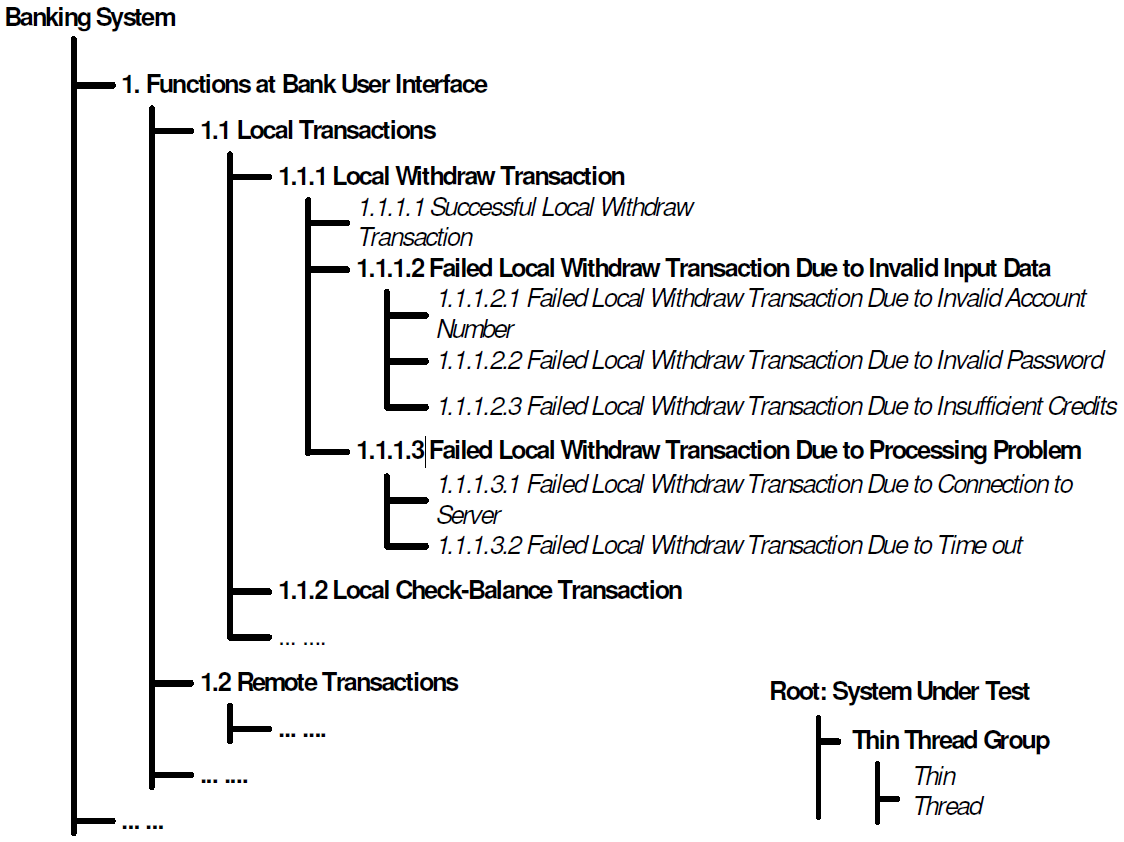
\includegraphics[scale=0.45]{img/Tsai2001ThinThreadTree.png}
    \caption{Een hypothetische thin-thread boom voor een bankiersapplicatie \autocite{Tsai2001}}
    \label{fig:tsaithinthreadtree}
\end{figure}

De relaties tussen thin-threads onderling worden bepaald door hoe hun uitvoeringspaden zich tot elkaar verhouden:

\begin{enumerate}
    \item ``Deel-geheel'': het pad van één thin-thread is deel van dat van een andere thin-thread
    \item ``Identiek'': de paden zijn identiek; ze delen condities of andere eigenschappen
    \item ``Onafhankelijk'': de thin-threads hebben volledig andere paden
\end{enumerate}

Ook de condities kennen een reeks mogelijke verhoudingen:

\begin{enumerate}
    \item ``Onafhankelijk'': één conditie kan zich met of zonder een andere voordoen
    \item ``Gekoppeld'': één conditie kan of zal de andere veroorzaken
    \item ``Wederzijds uitgesloten'': slechts één van beide kan zich in één situatie voordoen
    \item ``Gerelateerd'': twee condities worden in dezelfde thin-thread gebruikt of sluiten elkaar uit
\end{enumerate}

Bij het opstellen van \textbf{E2E test cases} op basis van deze techniek dienen eerst de de thin-threads, hun condities, hun mogelijke input- en outputgegevens, en de relaties tussen de thin-threads en de condities onderling vastgelegd te worden. De test cases worden vervolgens opgebouwd uit individuele thin-threads. Thin-threads kunnen na elkaar uitgevoerd worden (``sequencing''), herhaald worden (``looping'') en op basis van voorwaarden uitgevoerd worden (``conditioned execution'').

\begin{figure}[h!]
    \centering
    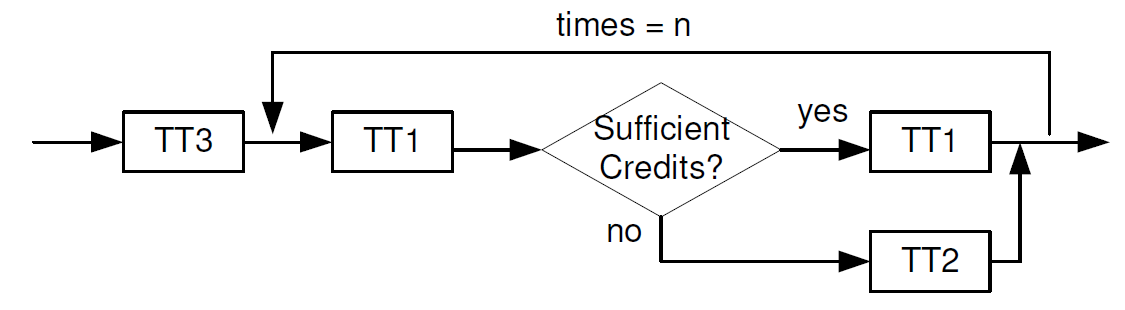
\includegraphics[scale=0.35]{img/Tsai2001ComplexTestScenario.png}
    \caption{Voorbeeld van een test case opgebouwd uit 3 verschillende thin-threads \autocite{Tsai2001}}
    \label{fig:tsaicomplexscenario}
\end{figure}

Om de test cases te vervolledigen tot reële gebruiksscenario's moet men ten slotte inputs kiezen op basis van de grenzen van de condities. Meestal gaat men \emph{grenswaarden} kiezen om te testen \autocite{Jorgensen2013}, maar dit kan ook door: de input \emph{willekeurig} te selecteren \autocite{Loo1988}, de mogelijke inputs in \emph{categorieën} te sorteren en daar representatieve data uit halen of door eenvoudigweg data uit de reële gebruiksomgeving te gebruiken (\emph{``usage-based testing''}) \autocite{Dyer1992}.

Thin threads steunen inherent op \textbf{reusability}, wat de opbouw van een test automatisatiesysteem niet alleen versnelt maar ook de kwaliteit en onderhoudbaarheid van het systeem ten goede komt \autocite{LombardHill2014}. De specifieke implementatie van thin threads is afhankelijk van het gebruikte framework. In de praktijk zullen dit vaak scripts zijn, hoewel elke vorm van hergebruik voordelig is \autocite{Madan2013} \autocite{Barrett2013}.

\subsubsection{Onderhoudbaarheid van een Test Automatisatiesysteem}

Het succes van een test automatisatieproject op de lange termijn is sterk afhankelijk van de onderhoudbaarheid van het systeem. Jim Holmes identificeert in zijn whitepaper ``Getting off on the Right Foot with Your Test Automation Project'' drie belangrijke problemen die de onderhoudbaarheid van web-based test automatisatiesystemen ondermijnen \autocite{Holmes2020}:

\begin{enumerate}
    \item Slecht gedefinieerde \textbf{``element locators''}.
    \item Synchronisatieproblemen bij \textbf{dynamische content}.
    \item Het niet consequent toepassen van \textbf{software engineering principes} zoals het \emph{Single Responsibility Principle} (SRP) en \emph{Don't Repeat Yourself} (DRY).
\end{enumerate}

De zogeheten ``locators'' laten toe dat het geautomatiseerde systeem elementen op een pagina kan vinden, bijvoorbeeld een input-element dat het syteem kan gebruiken om testdata in te voeren. Idealiter zijn deze locators:

\begin{itemize}
    \item \textbf{Flexibel}. Het gebruiken van het volledige pad van een element als locator is riskant; wijzigingen aan de structuur van pagina's maakt zulke locators snel onbruikbaar. Met unieke ID's, of tenminste vaste voor- en achtervoegsels voor bepaalde soorten elementen, kan men het gebruik van paden vermijden. Vaak is het ook mogelijk om elementen te selecteren op basis van één of meerdere criteria: types, klassen, inhoud, bovenliggende of onderliggende elementen, positie binnen een hiërarchie etc.
    \item \textbf{Gecentraliseerd}. Middels \emph{dictionaries} — die locators als sleutel/waarde-paren opslaan — of het \emph{page object pattern} — een recente techniek die pagina's als (objectgeoriënteerde) klassen met bijhorende attributen en methoden behandelt — kan men locators centraal beheren. Dit laat ook toe om locators te hergebruiken.
\end{itemize}

\begin{figure}[h!]
    \centering
    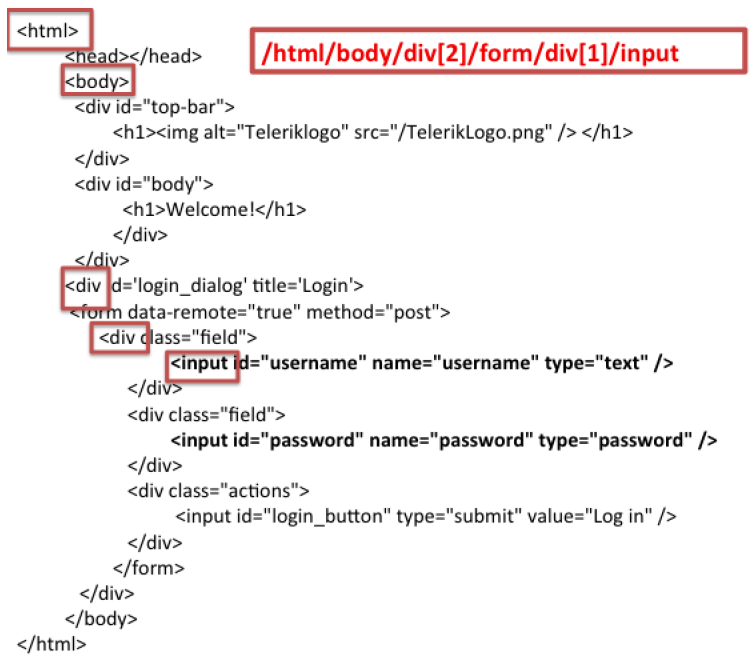
\includegraphics[scale=0.5]{img/Holmes2020XPath.PNG}
    \caption{Voorbeeld van een pad op een HTML-pagina \autocite{Holmes2020}}
    \label{fig:holmesxpath}
\end{figure}

De synchronisatieproblemen die optreden bij dynamische content worden vaak opgelost door expliciet te wachten tot aan bepaalde \emph{condities} voldaan wordt vooraleer verder te gaan naar de volgende stap. Een andere methode kan ontleend worden van Android Instrumentation testing: door gebruik te maken van het \emph{observer pattern} kan men wachten tot het gewenste resultaat beschikbaar is vooraleer verder te gaan met een test \autocite{Elye2018}. Dit vermijdt ook nodeloos wachten door gebruik te maken van een \emph{sleep}-functie.

Een andere belangrijke overweging is \textbf{test coverage} (testdekking): het aandeel van de code en de functionele vereisten zoals beschreven in de functionele specificatie dat in de (al dan niet geautomatiseerde) test cases gevalideerd wordt \autocite{Sheth2019}. Een dekkingsgraad van 100\% is niet in alle gevallen nodig om de kwaliteit van het opgeleverde softwareproduct te garanderen — sterker nog: eenmaal voorbij 90\% neemt de benodigde tijd om testen te implementeren voor het overblijvende deel sterk toe \autocite{Prause2017}.

\subsubsection{Beheer van Testdata}

Doorgaans worden testing frameworks ingedeeld in één van twee of drie groepen, op basis van hoe zij testdata beheren \autocite{Day2014} \autocite{Laukkanen2006}:

\begin{enumerate}
    \item \textbf{Data driven}. Dit type framework scheidt de testdata van de scripting logica door die eerste als sleutel-waarde paren op te slaan in een extern bestand (gaande van eenvoudige rekenbladen tot Open DataBase Connectivity). Testscenarios worden vaak met verschillende inputs (en corresponderende outputs) herhaald om alle mogelijk test cases af te dekken. Data driven frameworks leggen met andere woorden de nadruk op het verveelvuldigen van scenarios om de test coverage te vergroten.
    \begin{figure}[h!]
        \centering
        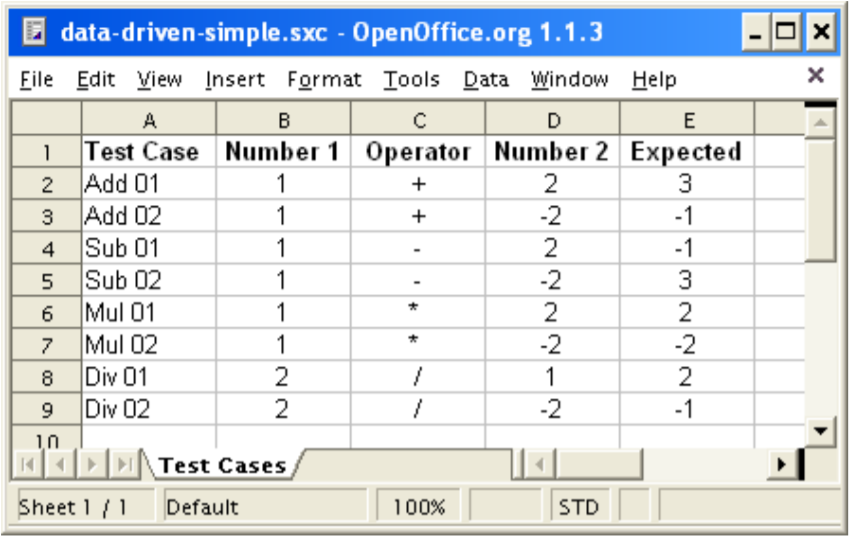
\includegraphics[scale=0.4]{img/Laukkanen2006DataDriven.PNG}
        \caption{Voorbeeld van sleutel-waarde paren die gebruikt worden binnen hetzelfde scenario, nl. de uitvoering van een binaire operatie \autocite{Laukkanen2006}.}
        \label{fig:laukkanendatadriven}
    \end{figure}
    \item \textbf{Keyword driven}. Keyword driven frameworks focusen zich vooral op hergebruik en onderhoudbaarheid van de testen. Stukken code, geïdentificeerd a.d.h.v \emph{keywords}, worden geïsoleerd in externe bestanden (data tables) samen met eventuele data/locators. Testscenarios worden vervolgens samengesteld door keywords aan elkaar te rijgen. Dit zorgt ook voor een grotere mate van afhankelijkheid van het framework zelf \autocite{Madan2013}.
        \begin{figure}[h!]
        \centering
        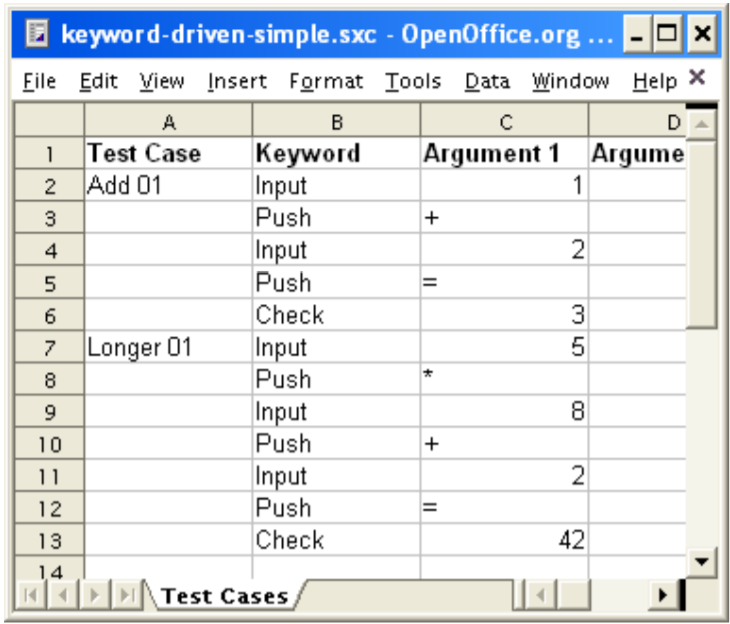
\includegraphics[scale=0.4]{img/Laukkanen2006KeywordDriven.PNG}
        \caption{Voorbeeld van test cases die opgebouwd worden uit keywords en bijhorende data \autocite{Laukkanen2006}.}
        \label{fig:laukkanenkeyworddriven}
    \end{figure}
    \item \textbf{Hybrid}. Hybride frameworks combineren bovenstaande technieken. De meeste mature frameworks lijken naar deze vorm te evolueren \autocite{Day2014}.
\end{enumerate}

\subsection{Overwegingen bij de Keuze voor een Test Automatisatiesysteem}

Test automatisatie vergt een substantiële initiële investering; analyse van de functionaliteit van de software, schrijven van testscripts, het introduceren van de tooling en het opleiden van personeel etc. \autocite{Kumar2016}. Het is dus van kritisch belang om een weloverwogen keuze te maken teneinde de kans op slagen van dergelijk project te maximaliseren. De volgende factoren zijn in het bijzonder belangrijk in acht te nemen:

\begin{itemize}
    \item \emph{De betrokken technologieën en omgevingen}. Het spreekt voor zich dat men voor het opzetten van test automatisatie anders te werk zal moeten gaan bij mainframe toepassingen dan voor webapplicaties. De beschikbare tooling zal ook afhankelijk zijn van de gebruikte technologieën (\cite{10.1145/1295014.1295062}).
    \item \emph{De beschikbare kennis}. Ervaring met een bepaald framework binnen het team is een sterke troef en vaak een doorslaggevende reden om een keuze te motiveren (\cite{Madan2013}).
    \item \emph{De lifecycle van de software}. Het te implementeren systeem dient te passen binnen het geplande levensverloop van de software zelf. Software waarvoor slechts een beperkt aantal toekomstige releases (of zelfs helemaal \emph{geen} toekomstige ontwikkeling) gepland is, zal niet gebaat zijn bij test automatisatie \autocite{Tiitinen2013}.
\end{itemize}

\section{e2e Testing Frameworks voor Angular}

~\cite{Singh2015}

\lipsum[4]

\subsection{Protractor}

\lipsum[6-7]

\subsection{Cypress}

\lipsum[3-4]

\subsection{UFT}

\lipsum[3-4]

\subsection{Behavior Driven Development Frameworks}

\lipsum[9]

\subsubsection{Mocha}

\lipsum[8-10]

\subsubsection{Jasmine \& Karma}

\lipsum[8-10]

\subsubsection{Cucumber}

\lipsum[8-10]